\section{System Overview}
\label{sec:art-overview}

The system architecture of the ART XRaaS is composed by different modules, each reflecting a phase of the creation process of an \gls{XR} experience (\autoref{fig:architecture}). The system is composed as follows:
\begin{itemize}
    \item A \textbf{Content Management System} (CMS) implements the \emph{assets upload phase}. It is a web application acting as entry point into the creation process, where designers of the \gls{XR} experience create or open an existing project and upload all the digital contents to be included in the next phases. It is served by a database to persist and retrieve assets, which can be 3D models (\textit{.fbx, .obj}), images or textures (\textit{.jpeg, .bmp, .png}), video clips (\textit{.mp4}), audio tracks (\textit{.mp3}), text documents (\textit{.txt}), QR Codes (described by their plain text content) and object-related operational entities (a \textit{menu}). Lastly, the application allows to categorize and label these assets, assigning them to different \emph{Scenes}.

    \item The \textbf{ART Editor} is involved in the \emph{interaction authoring phase}. It is a web application that, after retrieving all the assets already uploaded in the previous phase, allows to model in a canvas the interactions among these entities according to user inputs, using a "state-action-effect" paradigm typical of Finite State Machines (FSM). Indeed, the experience is described by a sequence of States connected by Actions, where each State contains different objects and each object has specific properties that can change. After modeling the interactions, the Editor allows to save the flow of the experience in a configuration file used in the next phase.
    
    \item A \textbf{\gls{HMD} Authoring Application} allows the \emph{on-site authoring phase}: during this phase the user, wearing a \gls{HMD}, opens the created project and a \emph{run-time engine} parses the configuration file exported in the previous phase; then, the application downloads all the assets from the CMS' database to proceed in the authoring process. During this phase the authors of the experience set each Scene, placing the assets in the virtual environment and configuring their properties such as position, scale and orientation; in the case of \gls{AR} authoring they map the coordinates of the physical environment with the digital one through \emph{Spacial Anchors}\footnote{\url{https://azure.microsoft.com/en-us/services/spatial-anchors/}} to persist the coordinates of digital contents with respect to real environment. 
    
    \item The on-site authoring phase is the last phase of the development process and, for complimentary, here we cite the last component of the system, that is the \textbf{Universal \gls{XR} Application Reader}. This is the final application for the end user (the tourist) that consists in a run-time engine responsible for the correct parse of the configuration file and rendering of the virtual environment. This application is available for both \glspl{HHD} and \glspl{HMD}, and in the latter case both for \gls{AR} and \gls{VR} devices.
\end{itemize}

\begin{figure}[h]
    \centering
    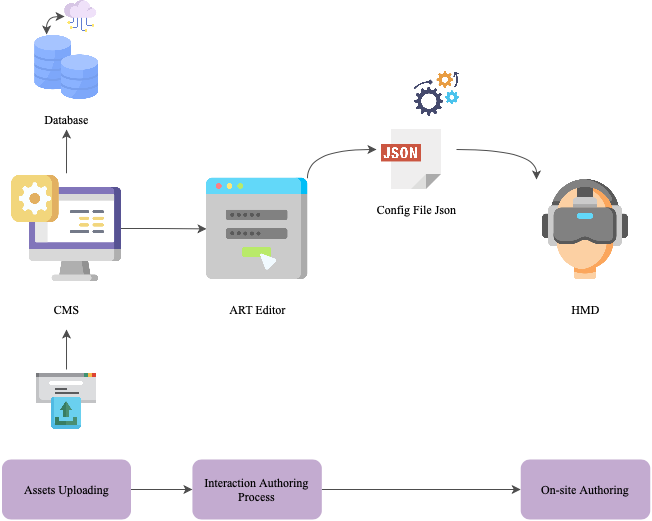
\includegraphics[width=\textwidth]{Figures/Editor/architecture.png}
    \caption{System Overview - Architecture}
    \label{fig:architecture}
\end{figure}

\subsection{ART User Journey}
\label{subsec:art-user-journey}

To give the reader a better understanding of the way the system works we provide a user journey considering the example of a cultural heritage site whose curators are interested in enhancing the experience of their visitors through \gls{XR} technologies. Their goals is to augment the information of the exhibits through virtual panels containing descriptions, historical videos, pictures and reconstruction models of the past; using the ART Framework it is only required some expertise in 3D content authoring to create the models, while the app development part is totally transparent to the user thanks to ART XRaaS. The user journey to develop the \gls{XR} experience would be the following:
\begin{enumerate}
    \item The user produces 3D models and gathers all the digital and multimedia assets contributing to the experience.
    \item The user accesses the web portal of the ART CMS and create a new project.
    \item The user upload all the assets on the CMS, then they define their properties such as names and labels to support the next development phase and, if necessary, cluster each of them in different scenes.
    \item The user opens the ART Editor and define the end user (tourist) interactions with the elements through a canvas and a "state – action – effect" paradigm.
    \item The user save the modelled experience and a configuration file is exported.
    \item The user, wearing a Microsoft HoloLens 2 \gls{HMD}, opens the exported configuration file using the on-site authoring application.
    \item The user decide to create an \gls{AR} application and scan the heritage site to place Spatial Anchors in it; to do so, they place the assets in the environment choosing their placement, size and orientation by manipulating these elements through \emph{gestures}.
    \item Finally, they save and publish the app that will be available for tourists, regardless of the \gls{AR} device used to augment their visit.
\end{enumerate}